Before the training procedure the data that was split before on two sets, non cancer and cancer, are getting resized so the training is more reliable and then they are put to new lists with their labels. After that the two lists are concatenated and split back, with the criterion of being an image or label into two different arrays (X, Y). At the final step the data was encoded using the one-hot encoding, to represent categorical variables as numerical values that is quite beneficial in the current project. Finally, the parameters of the training are ready and the only thing left is to separate the labeled data in to training and testing set, used for validation and testing (validation was avoided because of the small dataset). The percentage of split was chosen after many trials and the most efficient was the following :
\begin{figure}[H]
    \centering
    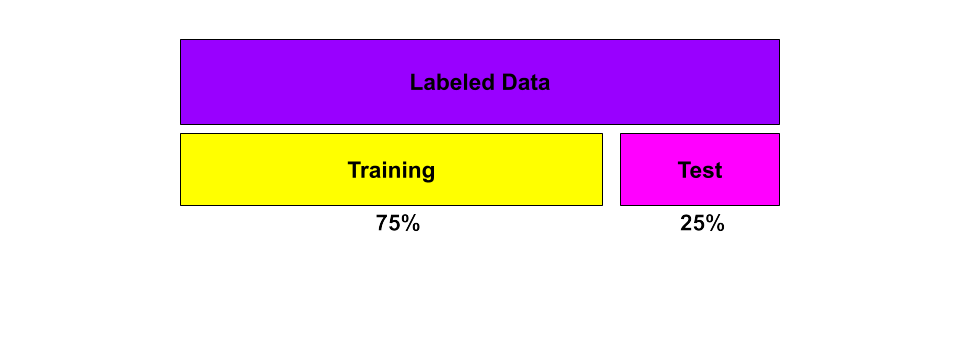
\includegraphics[width=0.6\textwidth]{Images/Data Split.png}
    \caption{Data Split}
    \label{fig:example}
\end{figure}